\documentclass{beamer}
\mode<presentation> {
    \usetheme{Copenhagen} \usecolortheme{whale}
    }
\usepackage{graphicx}
\usepackage{multicol}
\usepackage{subfig}

\setbeamersize{text margin left=3mm,text margin right=5mm }
\geometry{paperwidth=500pt, paperheight=300pt}
\usepackage{verbatim}
\graphicspath{{Images/}}
\title[Assignments 5]{MRAC SISO}
\author{Lorenzo Rossi Matricola: 0301285}
\begin{document}
\begin{frame}
	\titlepage{}
\end{frame}
\begin{frame}
	\begin{columns}[t]
		\begin{column}{.5\textwidth}
			\tableofcontents[sections={1-3}] % chktex 8
		\end{column}
		\hspace{-1cm}
		\begin{column}{.5\textwidth}
			\tableofcontents[sections={4-5}] % chktex 8
		\end{column}
	\end{columns}
\end{frame}
\begin{frame}
	\frametitle{Assignment 5}
	\section{Introduzione}
	Considerato il sistema del secondo ordine con funzione di trasferimento:\begin{equation}
        G(s)=k\frac{s+b_{0}}{s^{2}+a_{1}s+a_{0}}
    \end{equation}
    con \(k,b_{0}>0,a_{1},a_{0}\) costanti non note e modello di riferimento:\begin{equation}
        y_{m}=\frac{1}{s+1}r
    \end{equation}
    Sia \(\Lambda(s)=s+2\). Quindi, verificare he tutte le assunzioni per il design di un MRAC siano soddisfatte ed effettuare simulazioni del sistema a ciclo chiuso con MRAC assumento che \(b_{0}=2,a_{0}=5,a_{1}=-10,k=1,r=E_{1}\sin{(\omega_{1}t)}+E_{2}\sin{(\omega_{2}t)}, E_{1}\neq 0,E_{2}\neq 0, \omega_{1}\neq\omega{2} \)
\end{frame}
\begin{frame}
	\frametitle{Assunzioni}% chktex 8
	\section{Modello teorico}
	\subsection{Assunzioni Impianto}
    \begin{itemize}
        \item \textbf{Assunzioni dell'impianto} \(G(s)=k\frac{s+b_{0}}{s^{2}+a_{1}s+a_{0}}=k\frac{Z(s)}{R(s)}\):
        \begin{itemize}
            \item \(Z(s)\) è un polinomio monico di Hurwitz di grado m.
            Condizione necessaria affinché il polinomio \(s+b_{0}\) sia di Hurwitz se i coefficienti del polinomio siano tutti positivi. Quindi:\begin{equation}
                b_{1}>0, b_{0}>0
            \end{equation}
            Il polinomio è di Hurwitz;
            \item È noto un upper bound \(N\) di grado \(n\) di \(R(s)\): il limite è 2;
            \item È noto il grado relativo \(rd=n-m\) del sistema:\begin{equation}
                rd = 2- 1=1
            \end{equation}
            \item È noto il segno del guadagno ad alta frequenza \(k\): \(\forall k>0\)
        \end{itemize}
    \end{itemize}
\end{frame}
\begin{frame}
    \frametitle{Assunzioni}% chktex 8
    \subsection{Assunzioni del modello di riferimento}
    \begin{itemize}
        \item \textbf{Assunzioni del modello di riferimento} \(y_{m}=\frac{1}{s+1}r=k_{m}\frac{Z_{m}(s)}{R_{m}(s)} \):
        \begin{itemize}
            \item \(Z_{m}(s)\text{ e }R_{m}(s)\) sono polinomi monici di Hurwitz rispettivamente di grado \(m_{m},n_{m}\) con \(n_{m}\leq N\):\begin{align}
                m_{m}&=0\\
                n_{m}&=1\quad N=2\rightarrow  1\leq 2
            \end{align}
            \item Il grado relativo del modello di riferimento \(rd_{m}=n_{m}-m_{m}\) è tale che \(rd_{m}=rd\):\begin{equation}
                rd_{m}=1=rd
            \end{equation}
        \end{itemize}
    \end{itemize}
    Tutte le assunzioni sono verificate.
\end{frame}
\begin{frame}
	\frametitle{Modello teorico e implementazione Simulink}
	\section{Modello teorico e implementazione Simulink}
    \subsection{Regressore}
	\begin{itemize}
        \item \textbf{Regressore:}
        \begin{minipage}[t]{0.45\textwidth}
            \begin{equation}
                \dot{\omega_{1}}=F\omega_{1}+gu
            \end{equation}
            \begin{equation}
                \dot{\omega_{2}}=F\omega_{2}+gy
            \end{equation}
        \end{minipage}
        \begin{minipage}[t]{0.45\textwidth}
            \begin{figure}
                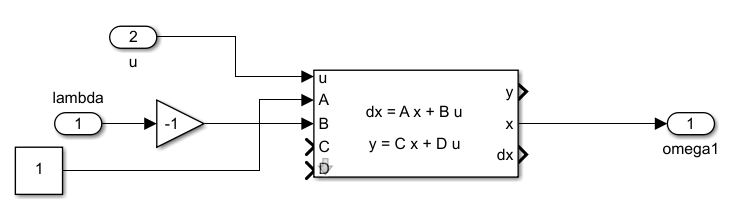
\includegraphics[scale=0.3]{2022-05-28-14-41-25.png}% chktex 8
                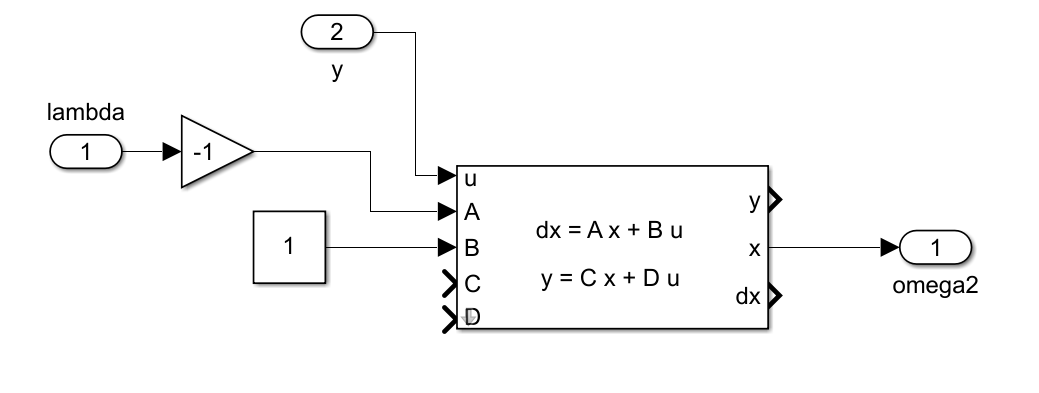
\includegraphics[scale=0.3]{2022-05-28-14-42-11.png}% chktex 8
            \end{figure}
        \end{minipage}
    \end{itemize}
\end{frame}
\begin{frame}
	\frametitle{Modello teorico e implementazione Simulink}
    \subsection{Controllore}
	\begin{itemize}
        \item \textbf{Controllore:}
        \begin{minipage}[t]{0.45\textwidth}
            \begin{equation}
                \theta=\begin{bmatrix}
                    \theta_{1}^{T}&\theta_{2}^{T}&\theta_{3}&c
                \end{bmatrix}^{T}
            \end{equation}
            \begin{equation}
                \omega=\begin{bmatrix}
                    \omega_{1}^{T}&\omega_{2}^T&y&y
                \end{bmatrix}^{T}
            \end{equation}\begin{equation}
                u=\hat{\theta}^T\omega
            \end{equation}
        \end{minipage}
        \begin{minipage}[t]{0.45\textwidth}
            \begin{figure}
                \centering
                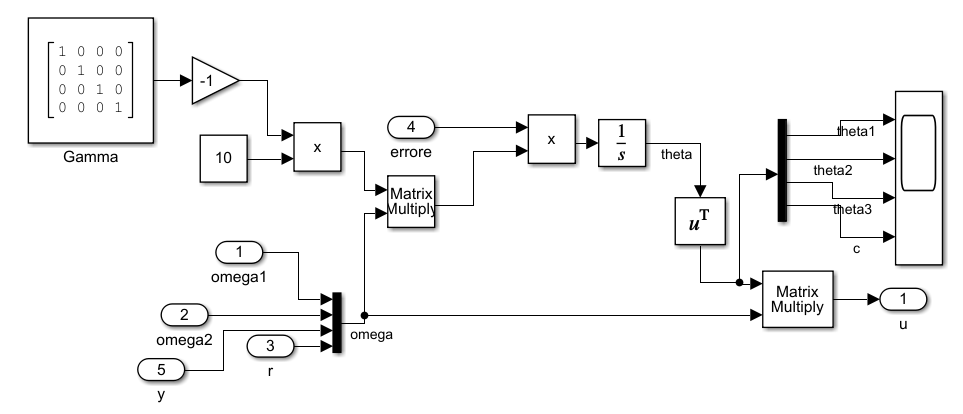
\includegraphics[scale=0.4]{2022-05-28-14-51-50.png}% chktex 8
            \end{figure}
        \end{minipage}
    \end{itemize}
\end{frame}
\begin{frame}
    \frametitle{Analisi}
    \section{Analisi}
    \begin{itemize}
        \item \textbf{Parametri:}\(E_{1}=1,E_{2}=1,\omega_{1}=1,\omega_{2}=5,F=diag(10)\)
    \end{itemize}
    \begin{figure}
        \centering
        \subfloat[\centering Intervallo totale]{{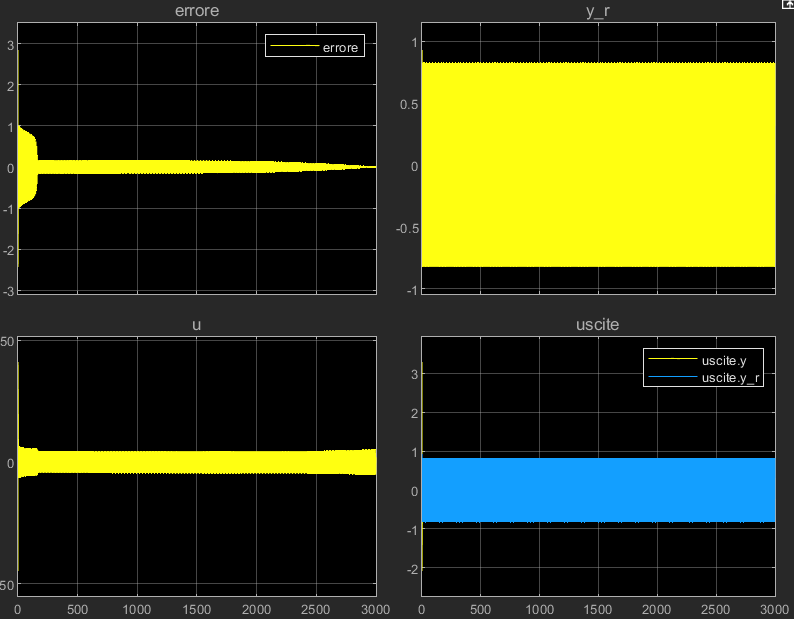
\includegraphics[scale=0.25]{2022-05-28-15-06-46.png}}}% chktex 8
        \hspace{0.2cm}
        \subfloat[\centering Ingrandimento a tempo finale]{{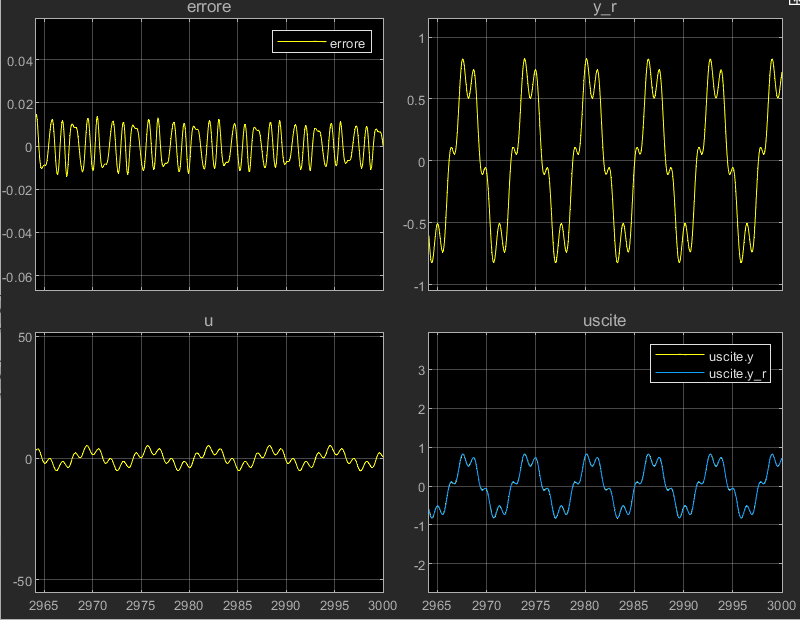
\includegraphics[scale=0.25]{2022-05-28-15-07-47.png}}}% chktex 8
        \hspace{0.2cm}
        \subfloat[\centering Theta]{{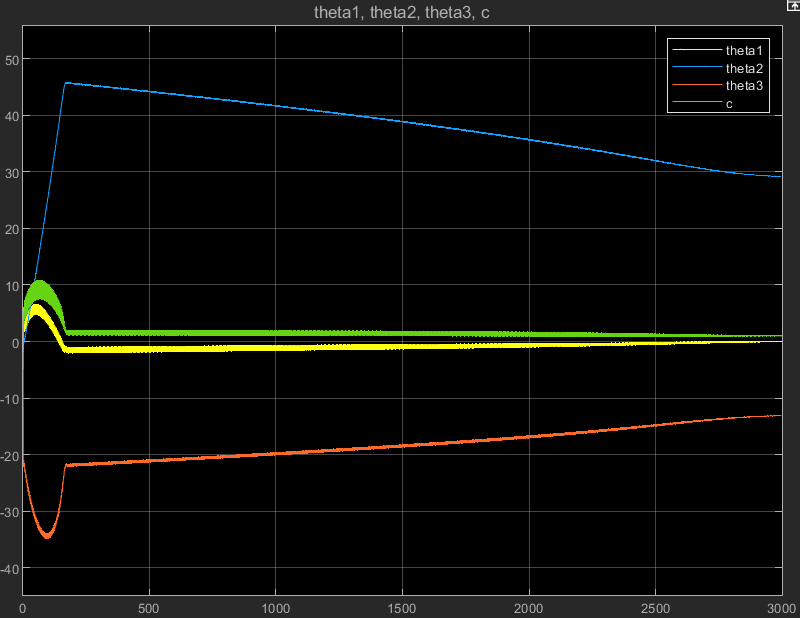
\includegraphics[scale=0.25]{2022-05-28-15-09-12.png}}}% chktex 8
    \end{figure}
\end{frame}
\begin{frame}
    \frametitle{Analisi}
    \begin{itemize}
        \item \textbf{Parametri:}\(E_{1}=1,E_{2}=1,\omega_{1}=1,\omega_{2}=5,F=diag(70)\)
    \end{itemize}
    \begin{figure}
        \centering
        \subfloat[\centering Intervallo totale]{{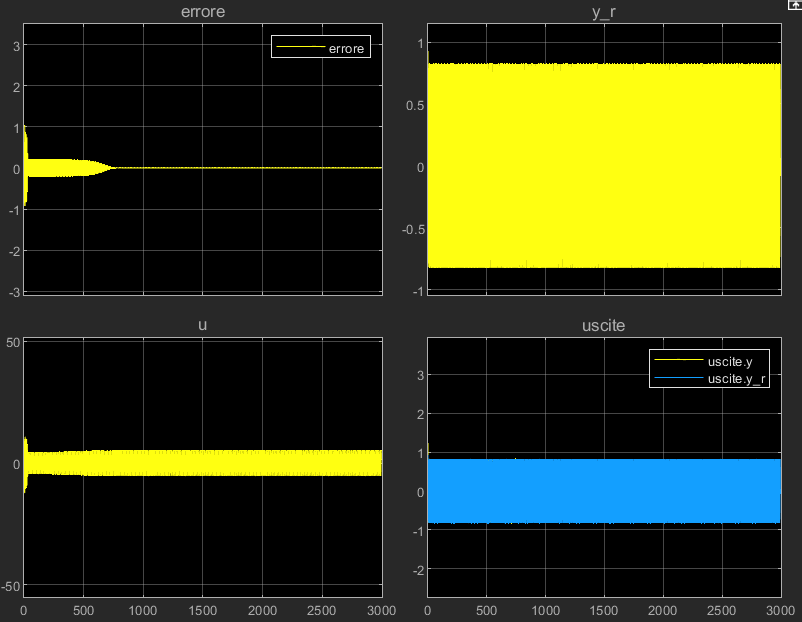
\includegraphics[scale=0.25]{2022-05-28-15-13-28.png}}}% chktex 8
        \hspace{0.2cm}
        \subfloat[\centering Ingrandimento a tempo finale]{{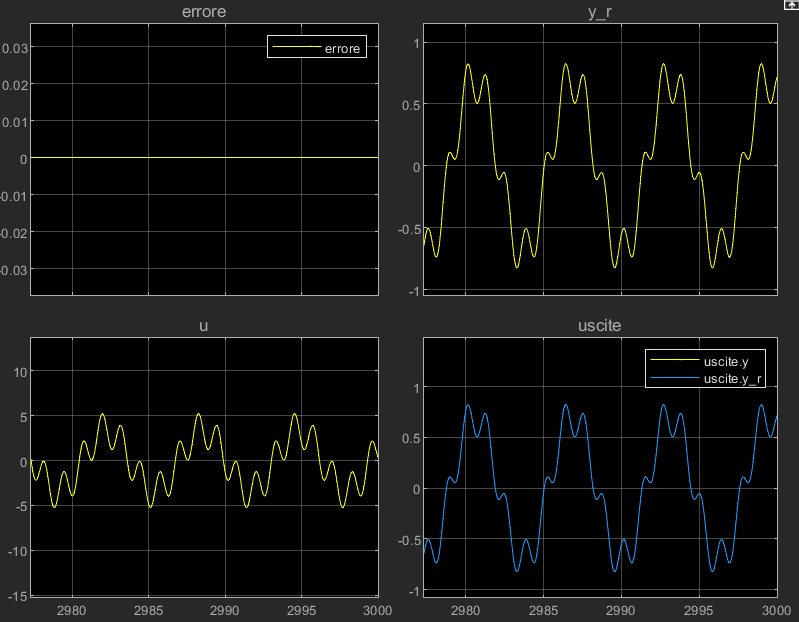
\includegraphics[scale=0.25]{2022-05-28-15-25-53.png}}}% chktex 8
        \hspace{0.2cm}
        \subfloat[\centering Theta]{{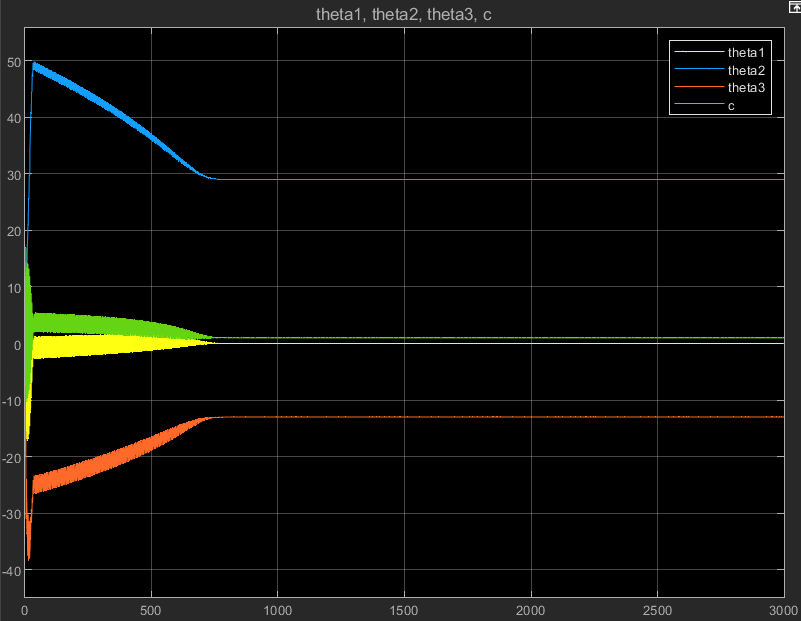
\includegraphics[scale=0.25]{2022-05-28-15-16-35.png}}}% chktex 8
    \end{figure}
\end{frame}
\begin{frame}
    \frametitle{Analisi}
    \begin{itemize}
        \item \textbf{Parametri:}\(E_{1}=7,E_{2}=5,\omega_{1}=1,\omega_{2}=5,F=diag(10)\)
    \end{itemize}
    \begin{figure}
        \centering
        \subfloat[\centering Intervallo totale]{{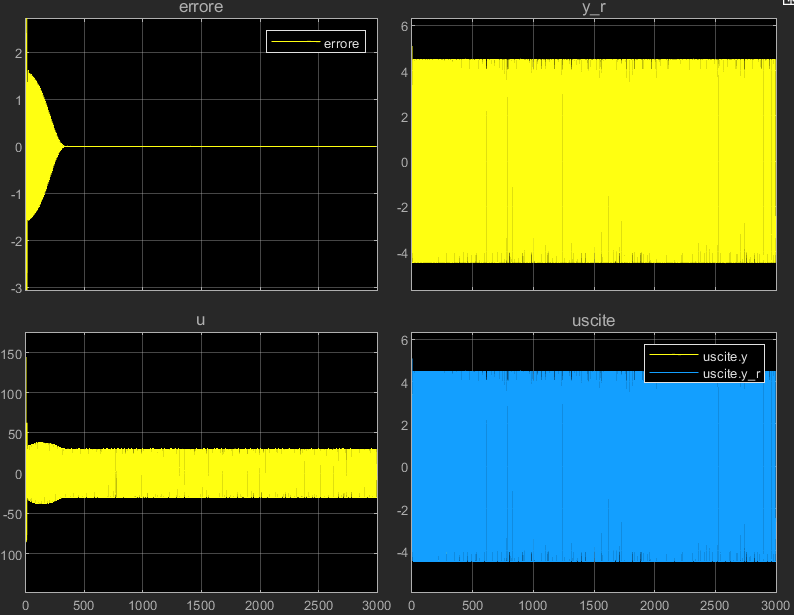
\includegraphics[scale=0.25]{2022-05-28-15-21-18.png}}}% chktex 8
        \hspace{0.2cm}
        \subfloat[\centering Ingrandimento a tempo finale]{{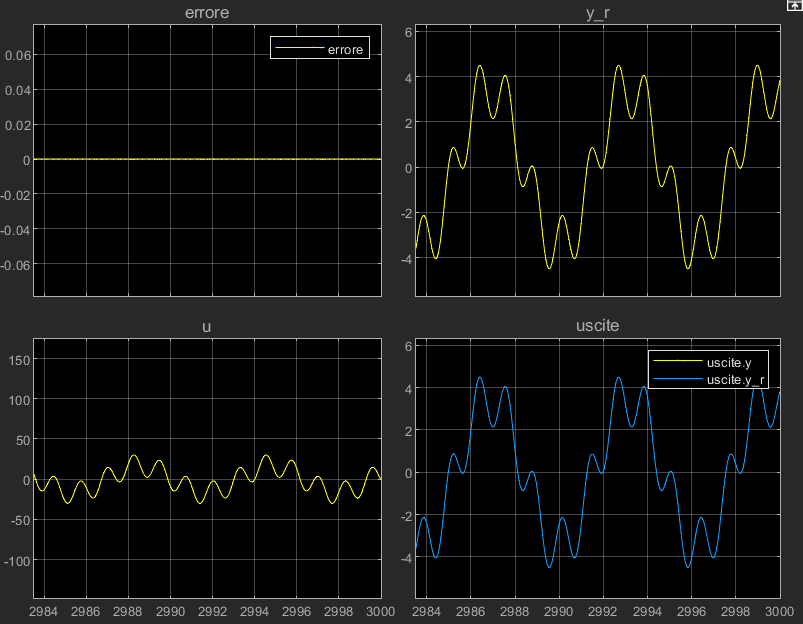
\includegraphics[scale=0.25]{2022-05-28-15-22-15.png}}}% chktex 8
        \hspace{0.2cm}
        \subfloat[\centering Theta]{{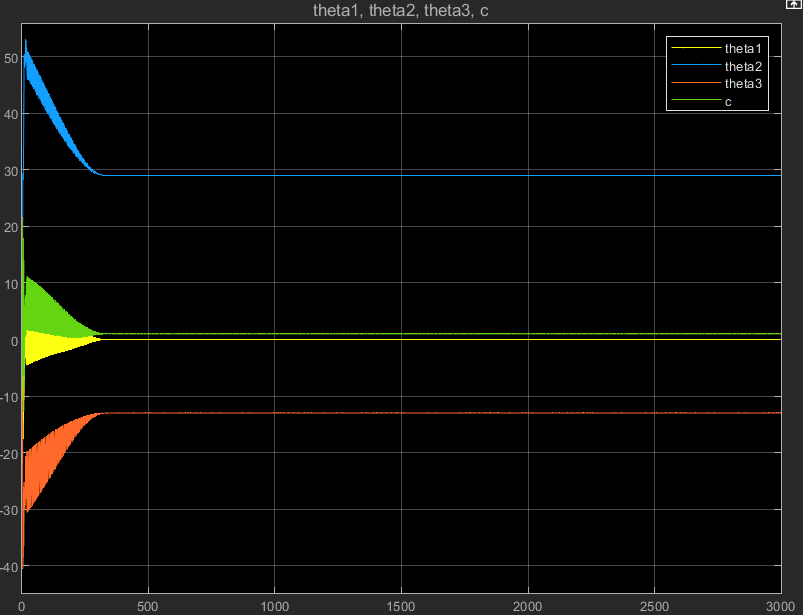
\includegraphics[scale=0.25]{2022-05-28-15-22-44.png}}}% chktex 8
    \end{figure}
\end{frame}
\begin{frame}
    \frametitle{Analisi}
    \begin{itemize}
        \item \textbf{Parametri:}\(E_{1}=7,E_{2}=5,\omega_{1}=1,\omega_{2}=5,F=diag(70)\)
    \end{itemize}
    \begin{figure}
        \centering
        \subfloat[\centering Intervallo totale]{{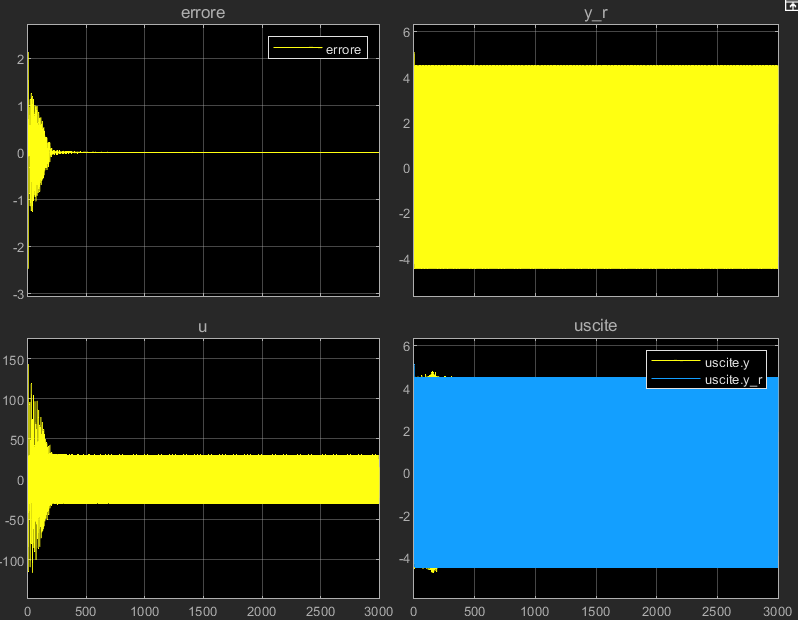
\includegraphics[scale=0.25]{2022-05-28-15-29-13.png}}}% chktex 8
        \hspace{0.2cm}
        \subfloat[\centering Ingrandimento a tempo finale]{{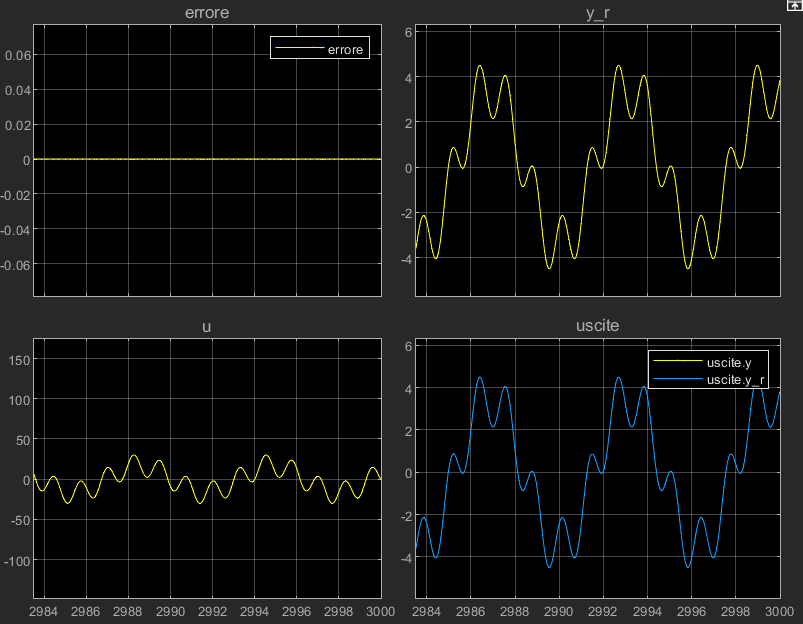
\includegraphics[scale=0.25]{2022-05-28-15-29-53.png}}}% chktex 8
        \hspace{0.2cm}
        \subfloat[\centering Theta]{{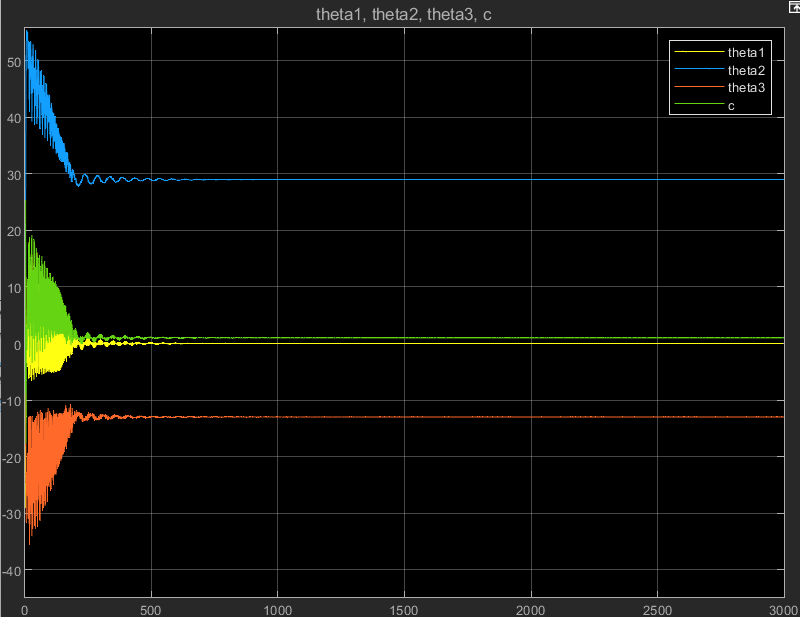
\includegraphics[scale=0.25]{2022-05-28-15-30-37.png}}}% chktex 8
    \end{figure}
\end{frame}
\begin{frame}
    \frametitle{Analisi}
    \begin{itemize}
        \item \textbf{Parametri:}\(E_{1}=1,E_{2}=1,\omega_{1}=5,\omega_{2}=10,F=diag(70)\)
    \end{itemize}
    \begin{figure}
        \centering
        \subfloat[\centering Intervallo totale]{{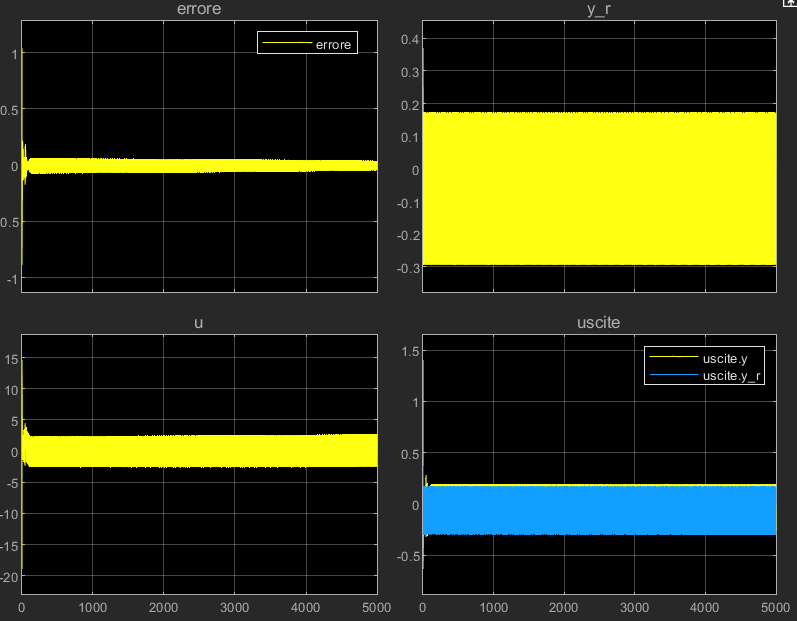
\includegraphics[scale=0.25]{2022-05-28-15-49-19.png}}}% chktex 8
        \hspace{0.2cm}
        \subfloat[\centering Ingrandimento a tempo finale]{{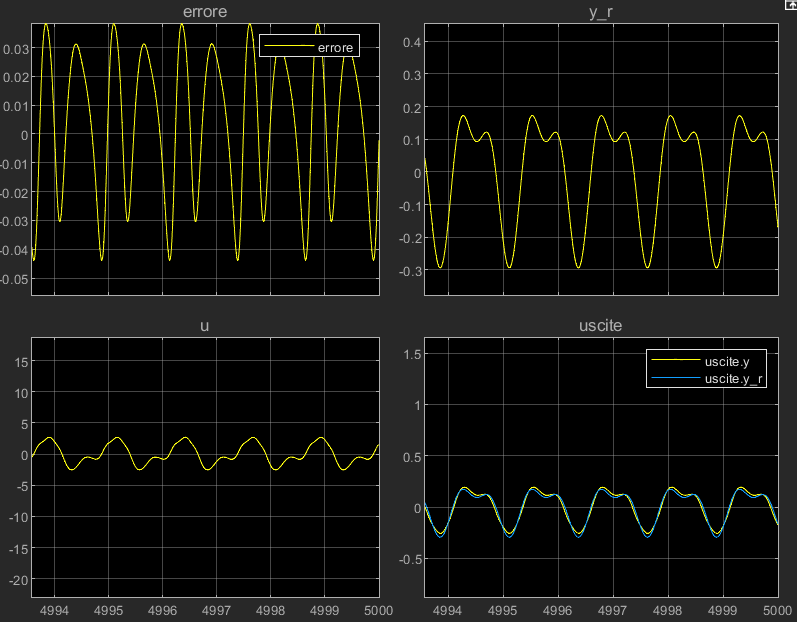
\includegraphics[scale=0.25]{2022-05-28-15-49-45.png}}}% chktex 8
        \hspace{0.2cm}
        \subfloat[\centering Theta]{{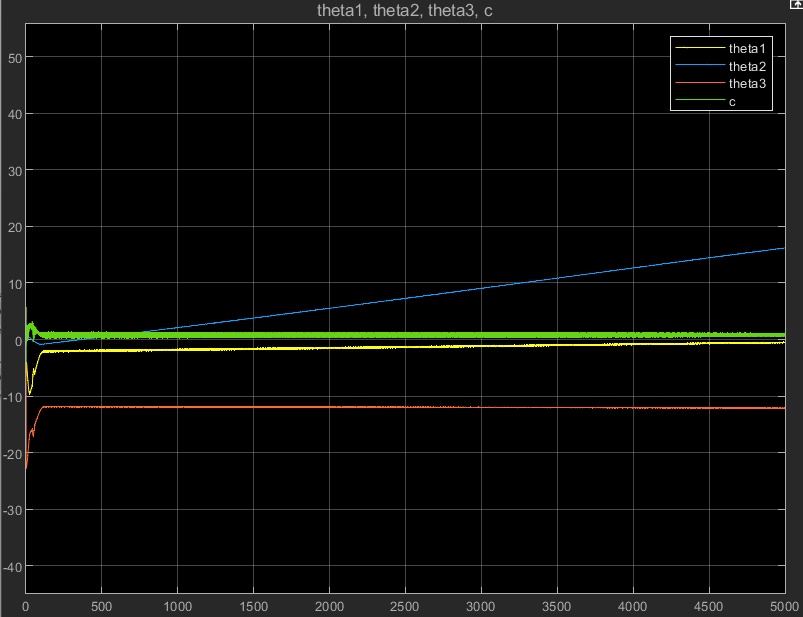
\includegraphics[scale=0.25]{2022-05-28-15-50-05.png}}}% chktex 8
    \end{figure}
\end{frame}
\begin{frame}
	\frametitle{Conclusioni}
	\section{Conclusioni}
    L'errore, come ci aspettimo dalla teoria, tende asintoticamente a zero nel tempo di simulazione scelte. Ne fa eccezione l'ultima simulazione proposta in cui, sebbene l'errore sia dimiunuito, non è giunto ancora a 0. Inoltre, i risultati proposti variano notevolemente in base alla scelta in base alle frequenze, le ampiezze scelte ed ai valori di \(\Gamma \). In particolare, a valori bassi di \(\Gamma \) corrisponde un transitorio più regolare con tempi di risposta maggiorni e con stime dei parametri più lente; al contrario, per valori alti di \(\Gamma \) si ha un transitorio meno regolare, con tempi di risposta minori, azioni di controllo più intense e stime dei parametri più veloci.
    Nell'ultima simulazione la non convergenza dei parametri e dell'errore può esser dovuto ad un problema numerico o ad una instabilità dei poli del sistema.
\end{frame}
\end{document}